\subchapter{First Yocto Project build}{Your first dive into Yocto
Project and its build mechanism}

During this lab, you will:
\begin{itemize}
  \item Set up an OpenEmbedded environment
  \item Configure the project and choose a target
  \item Build your first Poky image
\end{itemize}

\section{Setup}

Before starting this lab, make sure your home directory is not
encrypted. OpenEmbedded cannot be used on top of an eCryptFS file
system due to limitations in file name lengths.

Go to the \code{$HOME/yocto-labs/} directory.

Install the required packages:
\begin{verbatim}
sudo apt-get install bc build-essential chrpath cpio diffstat gawk git python texinfo wget
\end{verbatim}

\section{Download Yocto}

Download the \code{krogoth} version of Poky and apply a custom patch:
\begin{verbatim}
git clone git://git.yoctoproject.org/poky.git
cd $HOME/yocto-labs/poky
git checkout -b krogoth-15.0.1 krogoth-15.0.1
git am $HOME/yocto-labs/0001-Fix-lab.patch
\end{verbatim}

Return to your project root directory (\code{cd $HOME/yocto-labs/})
and download the OpenEmbedded TI layer:
\begin{verbatim}
git clone git://git.yoctoproject.org/meta-ti.git
cd $HOME/yocto-labs/meta-ti
git checkout -b ti2016.03 ti2016.03
git am $HOME/yocto-labs/0001-Simplify-linux-ti-staging-recipe.patch
\end{verbatim}

\section{Set up the build environment}

Check you're using Bash. This is the default shell when using Ubuntu.

Export all needed variables and set up the build directory:
\begin{verbatim}
cd $HOME/yocto-labs/poky/
source oe-init-build-env
\end{verbatim}

You must specify which machine is your target. By default it
is \code{qemu}. We need to build an image for a \code{beaglebone}.
Update the \code{MACHINE} configuration variable accordingly. Be
careful, \code{beaglebone} is different from the \code{beagleboard}
machine!

Also, if you need to save disk space on your computer you can add \code{INHERIT
+= "rm_work"} in the previous configuration file. This will remove the
package work directory once a package is built.

Don't forget to make the configuration aware of the TI layer. Edit the
layer configuration file (\code{$BUILDDIR/conf/bblayers.conf}) and append the
full path to the \code{meta-ti} directory to the \code{BBLAYERS} variable.

\section{Build your first image}

Now that you're ready to start the compilation, simply run:
\begin{verbatim}
bitbake core-image-minimal
\end{verbatim}

Once the build finished, you will find the output images under
\code{$BUILDDIR/tmp/deploy/images/beaglebone}.

\section{Set up the SD card}

In this first lab we will use an SD card to store the bootloader, kernel and
root filesystem files. Before copying the images on it, we first need to set up the
partition layout. You will find a bash script to do so, under
\code{$HOME/yocto-labs/script/}.

Execute it:
\begin{verbatim}
umount /dev/mmcblk0*
sudo ./format_sdcard.sh /dev/mmcblk0
\end{verbatim}

Once this is finished, remove the SD card, then insert it again, it
should automatically be mounted.

You can now copy the two U-Boot stages, the Linux kernel image and the compiled
device tree in the \code{boot} partition.
\begin{verbatim}
cp $BUILDDIR/tmp/deploy/images/beaglebone/{MLO,u-boot.img,zImage} \
  /media/$USER/boot
cp $BUILDDIR/tmp/deploy/images/beaglebone/zImage-am335x-boneblack.dtb \
  /media/$USER/boot/dtb
\end{verbatim}

Now uncompress the generated rootfs in the second partition with the
following \code{tar} command:
\begin{verbatim}
sudo tar xpf $BUILDDIR/tmp/deploy/images/beaglebone/\
  core-image-minimal-beaglebone.tar.gz -C /media/$USER/rootfs
sync
\end{verbatim}

\section{Setting up serial communication with the board}

The Beaglebone serial connector is exported on the 6 pins close to one
of the 48 pins headers. Using your special USB to Serial adapter provided
by your instructor, connect the ground wire (blue) to the pin closest
to the power supply connector (let's call it pin 1), and the \code{TX} (red)
and \code{RX} (green) wires to the pins 4 (board \code{RX}) and
5 (board \code{TX})\footnote{See
\url{https://www.olimex.com/Products/Components/Cables/USB-Serial-Cable/USB-Serial-Cable-F/}
for details about the USB to Serial adapter that we are using.}.

You always should make sure that you connect the \code{TX} pin of the cable
to the \code{RX} pin of the board, and vice-versa, whatever the board and
cables that you use.

\begin{center}
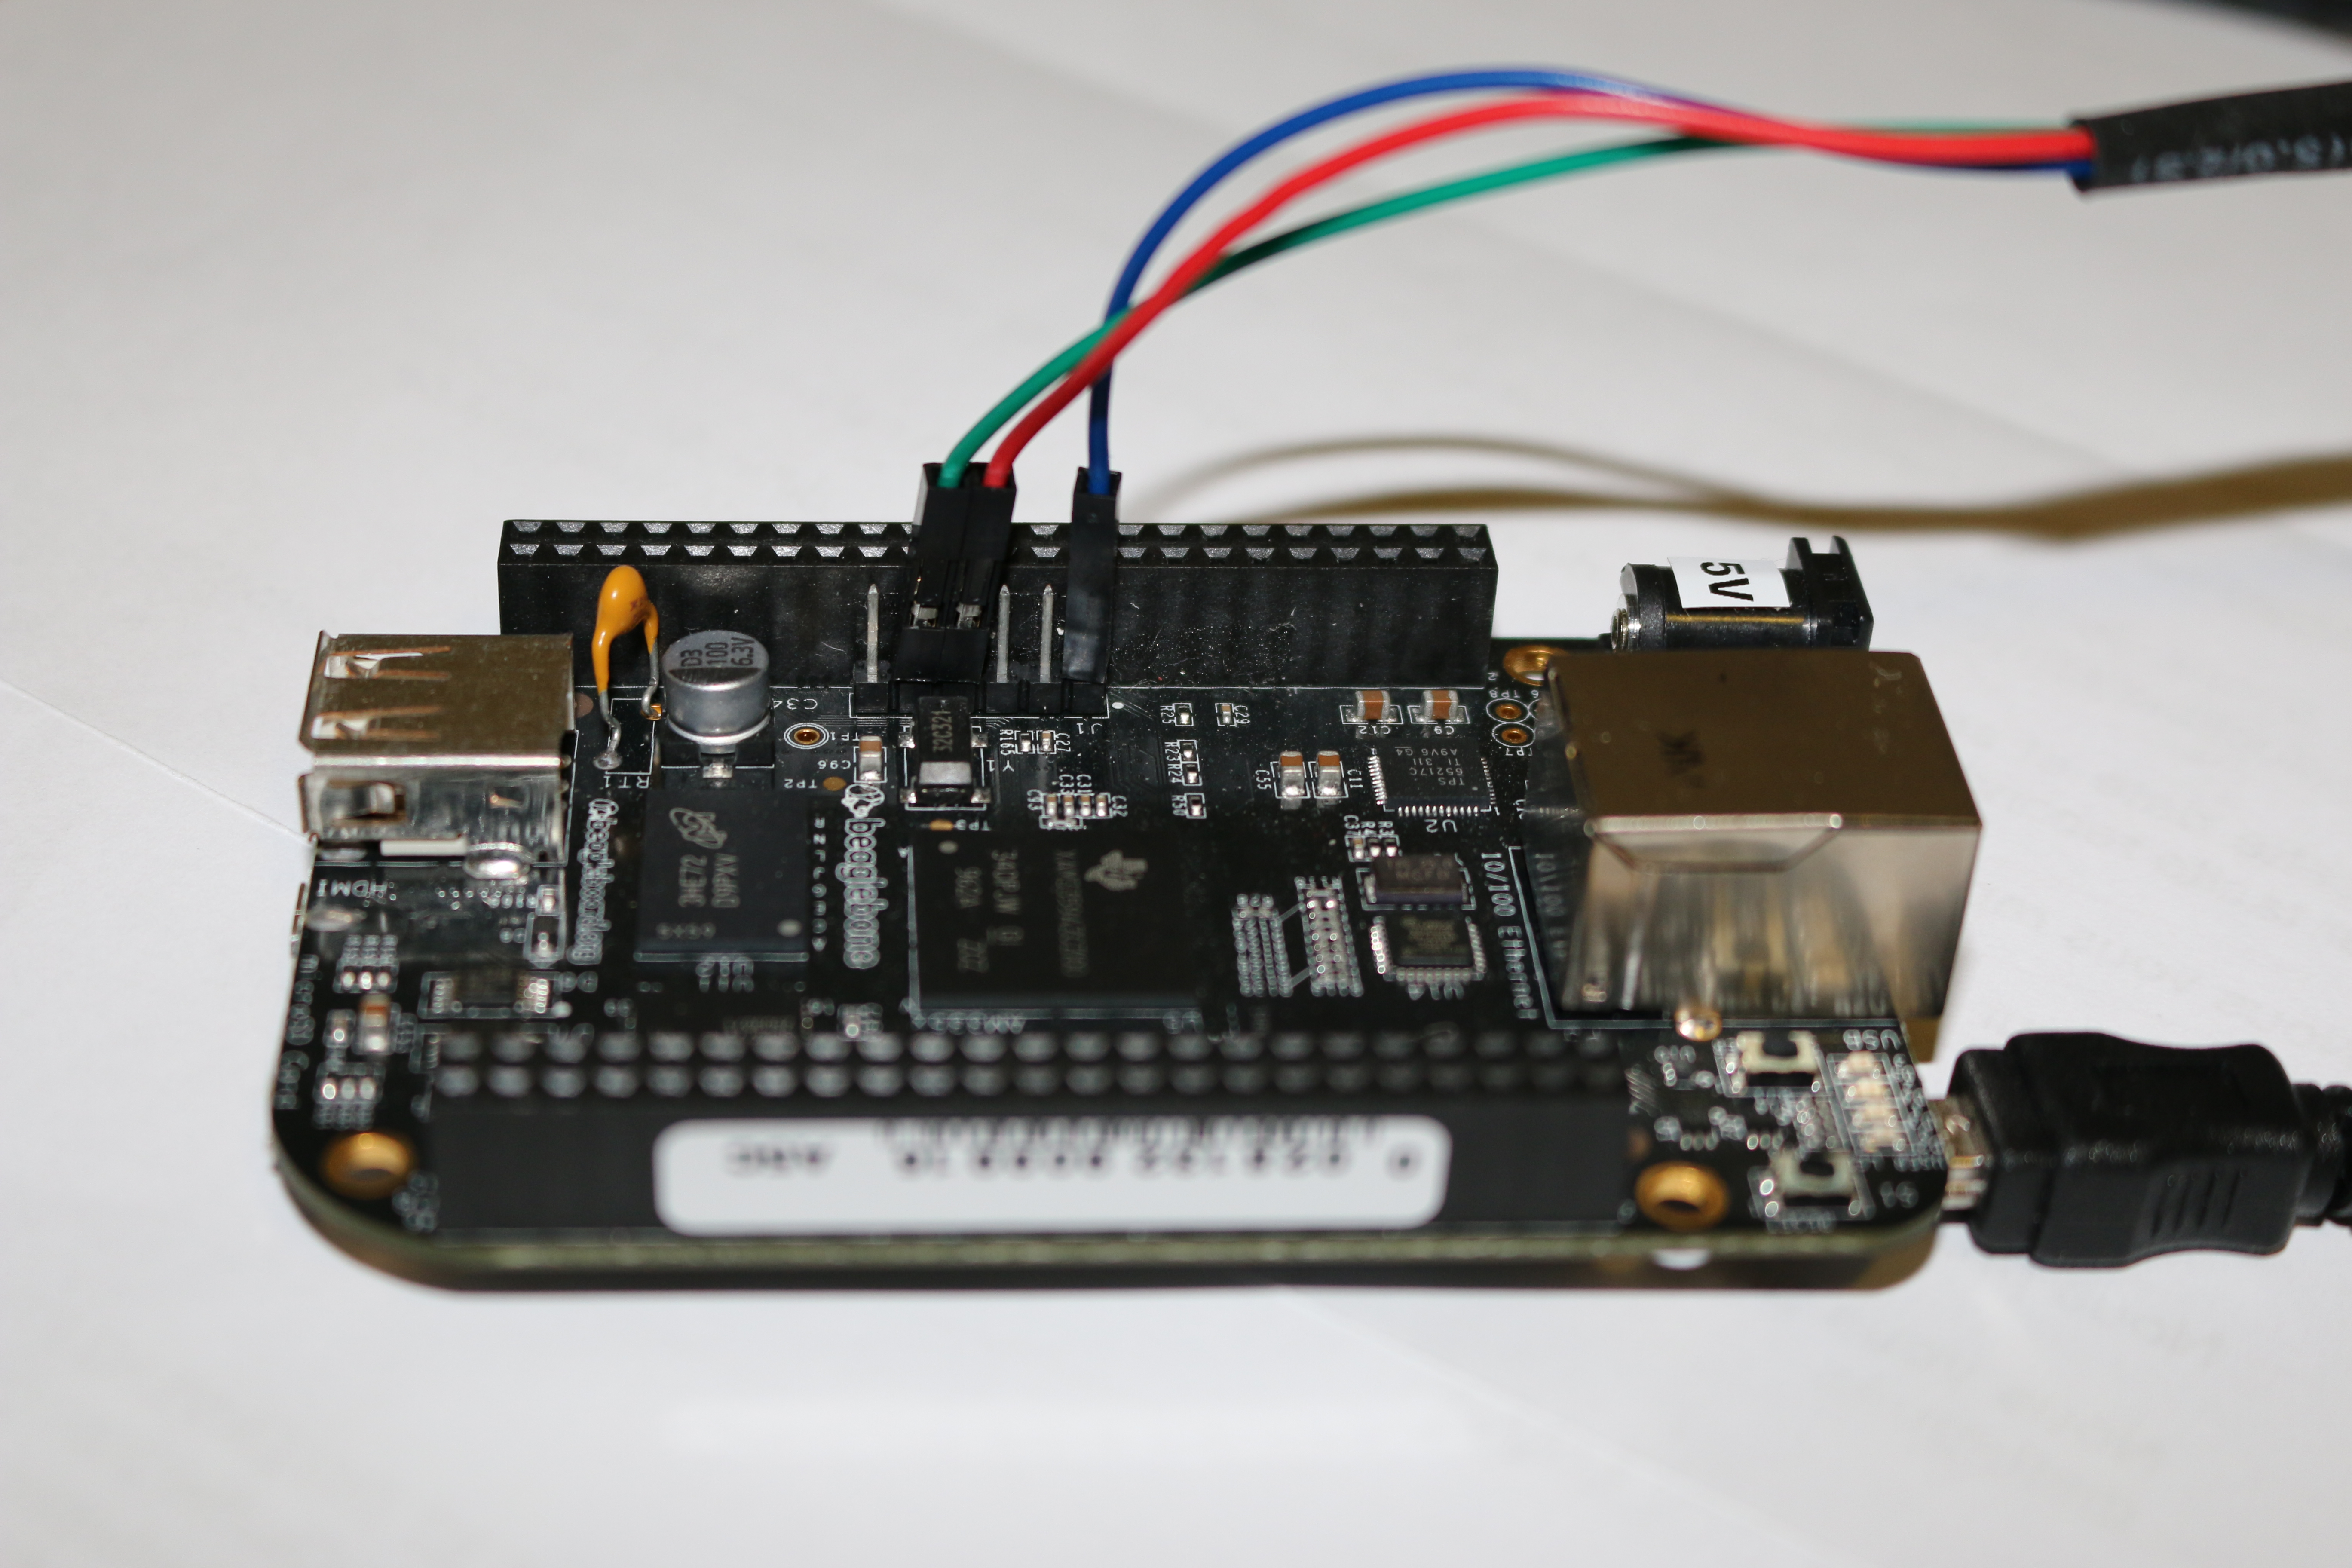
\includegraphics[width=8cm]{labs/yocto-first-build/beaglebone-black-serial-connection.jpg}
\end{center}

Once the USB to Serial connector is plugged in, a new serial port
should appear: \code{/dev/ttyUSB0}.  You can also see this device
appear by looking at the output of \code{dmesg}.

To communicate with the board through the serial port, install a
serial communication program, such as \code{picocom}:

\begin{verbatim}
sudo apt-get install picocom
\end{verbatim}

If you run \code{ls -l /dev/ttyUSB0}, you can also see that only
\code{root} and users belonging to the \code{dialout} group have
read and write access to this file. Therefore, you need to add your user
to the \code{dialout} group:

\begin{verbatim}
sudo adduser $USER dialout
\end{verbatim}

You now need to log out and log in again to make the new group
visible everywhere.

Now, you can run \code{picocom -b 115200 /dev/ttyUSB0}, to start serial
communication on \code{/dev/ttyUSB0}, with a baudrate of \code{115200}. If
you wish to exit \code{picocom}, press \code{[Ctrl][a]} followed by
\code{[Ctrl][x]}.

There should be nothing on the serial line so far, as the board is not
powered up yet.

\section{Configure the U-Boot environment and boot}

Insert the SD card in the dedicated slot on the BeagleBone Black. Press the S2
push button (located just above the previous slot), plug in the USB cable and
release the push button. You should see boot messages on the console.

Stop the boot process when you see \code{Press SPACE to abort autoboot} to
access the U-Boot command line.

In order to boot properly, you need to set up some configuration variables to
tell the bootloader how to load the Linux kernel. In the U-Boot command-line,
set the following variables:
\begin{verbatim}
setenv bootcmd 'mmc rescan; fatload mmc 0 0x80200000 zImage; fatload mmc 0
0x82000000 dtb; bootz 0x80200000 - 0x82000000'
setenv bootargs 'console=ttyO0,115200 root=/dev/mmcblk0p2 rw'
saveenv
\end{verbatim}

Finally you can start the kernel using the U-Boot command \code{boot}. Wait
until the login prompt, then enter \code{root} as user. Congratulations! The
board has booted and you now have a shell.
